%%%%%%%%%%%%%%%%%%%%%%%%%%%%%%%%%%%%%%%%%%%%%%%%%%%%%%%%%%%%%%%%%%%%%
%%        Copyright (c) 2021 Carsten Wulff Software, Norway
%% %%%%%%%%%%%%%%%%%%%%%%%%%%%%%%%%%%%%%%%%%%%%%%%%%%%%%%%%%%%%%%%%%%%
%% Created       : wulff at 2021-6-13
%% %%%%%%%%%%%%%%%%%%%%%%%%%%%%%%%%%%%%%%%%%%%%%%%%%%%%%%%%%%%%%%%%%%%
%%  The MIT License (MIT)
%%
%%  Permission is hereby granted, free of charge, to any person obtaining a copy
%%  of this software and associated documentation files (the "Software"), to deal
%%  in the Software without restriction, including without limitation the rights
%%  to use, copy, modify, merge, publish, distribute, sublicense, and/or sell
%%  copies of the Software, and to permit persons to whom the Software is
%%  furnished to do so, subject to the following conditions:
%%
%%  The above copyright notice and this permission notice shall be included in all
%%  copies or substantial portions of the Software.
%%
%%  THE SOFTWARE IS PROVIDED "AS IS", WITHOUT WARRANTY OF ANY KIND, EXPRESS OR
%%  IMPLIED, INCLUDING BUT NOT LIMITED TO THE WARRANTIES OF MERCHANTABILITY,
%%  FITNESS FOR A PARTICULAR PURPOSE AND NONINFRINGEMENT. IN NO EVENT SHALL THE
%%  AUTHORS OR COPYRIGHT HOLDERS BE LIABLE FOR ANY CLAIM, DAMAGES OR OTHER
%%  LIABILITY, WHETHER IN AN ACTION OF CONTRACT, TORT OR OTHERWISE, ARISING FROM,
%%  OUT OF OR IN CONNECTION WITH THE SOFTWARE OR THE USE OR OTHER DEALINGS IN THE
%%  SOFTWARE.
%%
%%%%%%%%%%%%%%%%%%%%%%%%%%%%%%%%%%%%%%%%%%%%%%%%%%%%%%%%%%%%%%%%%%%%%%


\documentclass[technote,10pt,a4paper]{IEEEtran}


\usepackage[final]{graphicx}
\ifCLASSINFOpdf
\graphicspath{{.}}
\DeclareGraphicsExtensions{.pdf}
\else
\graphicspath{{.}}
\DeclareGraphicsExtensions{.eps}
\fi
\usepackage{wrapfig}
\usepackage{upgreek}
\usepackage{amssymb,amsmath}
\usepackage{cite}
\usepackage{verbatim}
\usepackage{listings}
\usepackage{xcolor}
\usepackage{flafter}
\usepackage{booktabs}
\usepackage{url}
\usepackage{textcomp}
\usepackage{dirtytalk}
\definecolor{armygreen}{rgb}{0, 0.5, 0}
\newcommand{\missing}[1]{{ #1}}
\newcommand{\edit}[1]{{ #1}}
\newcommand{\secedit}[1]{{ #1}}
\newcommand{\deleted}[1]{{ #1}}
\newcommand{\moved}[1]{{ #1}}
\newcommand{\eqn}[1]{
  \begin{equation}
    #1
  \end{equation}}

\newcommand{\qt}[1]{
  \begin{quote}
    \small
    \textit{
      #1
     }
   \end{quote}}


 \graphicspath{ {./} }

% -----------------------------------------------------------------
% Header
% -----------------------------------------------------------------
\begin{document}
\bibliographystyle{IEEEtran}
\title{Why learn design of integrated circuits?}
\author{Carsten~Wulff, \textit{2021-06-13}, v0.1.0 }
\maketitle

% -----------------------------------------------------------------
% Abstract
% -----------------------------------------------------------------
\begin{abstract}
I explain what you'll learn in Design of Integrated Circuits, why integrated
circuits are used, why I work on them, and how we'll teach you about integrated circuits.
\end{abstract}

% -----------------------------------------------------------------
\section{Introduction}
% -----------------------------------------------------------------
The manufacture of integrated circuits is complicated, and only a handful of
companies -- TSMC, Samsung, Globalfoundries, and maybe a few others -- have the the capital and capability push
the cutting edge. Most of us in the IC industry work in companies called fabless design houses.
We design ICs but we don't manufacture them.

Integrated circuits are everywhere, in every cell phone, almost every toy,
computer, washing machine, fridge, and electric scooter. A modern car has hundreds.
Someone has to know how to make these integrated circuits. Today, that is me,
and my colleagues. Tomorrow, it will be some of you. You're at a disadvantage though. The
circuits are more complex and complicated than 60 years ago, and you may need to invent new
methods to deal. I can help you learn what you need to know
to make today's integrated circuits, but I can't teach you what you need to
invent the integrated circuits of tomorrow.

I can promise you, however, that what I'll help you learn is not wasted. In this
course we deal with physics and the fundamental components of ICs. Although the details might change,
the physical properties of transistors have remained the same for more than 70
years, since Brittain, Bardeen and Shockley discovered the first
\cite{bbs47}.

% -----------------------------------------------------------------
\section{Why}
% -----------------------------------------------------------------
Why make integrated circuits, and why learn them? For me, it's this. I use my
computer to design a piece of an integrated circuit. Maybe it takes me 6
months. The pieces are combined into a IC. Then, it might take a year or two
until it goes into volume production. Why so long? The bane of ICs is
variability, no transistor, resistor, capacitor, diode, inductor are the same.
We have to make sure that each IC works by test over temperature, voltage,
humidity, impact, age, electrostatic discharge. Google 'jedec esd', 'jedec
htol', or 'jedec hast' and you'll see what I mean. Testing takes time.

When an IC is in volume production our customers can design them into their
products. That takes time. But, after 5 years there can be hundreds of customers selling end products back to
me, using the integrated circuit I worked on.
The work I've done, the new circuit I've made, the tools I put into
the hands of my customers, may have made the world better. Maybe by pushing
people to get off the couch (step counters and heart rate monitors), improving
everyday life of diabetics (smart insulin pump), or reducing energy consumption
(smart lights, and smart buildings). I find that rewarding, especially when I
think of the billions of copies of my work that is out there.

I believe, that integrated circuits, is one of the few industries where you can make
something in Trondheim, and affect the fate of the whole world.

% -----------------------------------------------------------------
\section{How}
% -----------------------------------------------------------------


Imagine the computer
mouse you bought, inside the mouse is a printed
circuit board (PCB), and on that printed circuit board are multiple integrated
circuits. One for universal serial bus (USB), one for charging a battery, one for laser
sensor, one for communication. In addition, capacitors, crystals, inductors,
resistors, diodes, electrostatic discharge protection, ground planes, antennas,
and so much more.

The IC in figure \ref{fig_qfn} is a micro-controller
with a Bluetooth Low Energy radio, which in a mouse is used for communication
with a PC. The pins in black are digital inputs/outputs, the green are analog, the red are power, and blue is the ground connection.
The digital input/outputs are controlled via the micro-controller, or peripherals -- SPI, I2C,
UART. The analog pins  need external circuits like, crystal
(XC1, XC2), inductor and capacitor (DCC), matching network and antenna (ANT).
The power supply can come from a battery (VDD), while the DEC pins are the
outputs of internal voltage regulators.

You may ask -- will I learn everything on the inside in this course -- and the
answer is no. How can I help you learn about the millions of digital
gates, and thousand schematic pages in this integrated circuit when you may not
have understood the transistor yet? We must start with the basics, the
technology, devices, and fundamental blocks.  I can promise though, that if you choose take courses like
analog CMOS, digital design, digital communication, digital signal processing,
and advanced integrated circuits (my course), you will start to understand. Fair
warning, very few people master all areas of integrated circuit design, I choose to
focus on analog, others choose digital, or signal processing. Most of you will have too choose. A few of you may have the hubris
to think that you can learn everything. I like hubris.

I need you to trust me that I will help you learn the fundamentals. A
foundation to build on for future years.


\begin{figure}[tb]
  \centerline{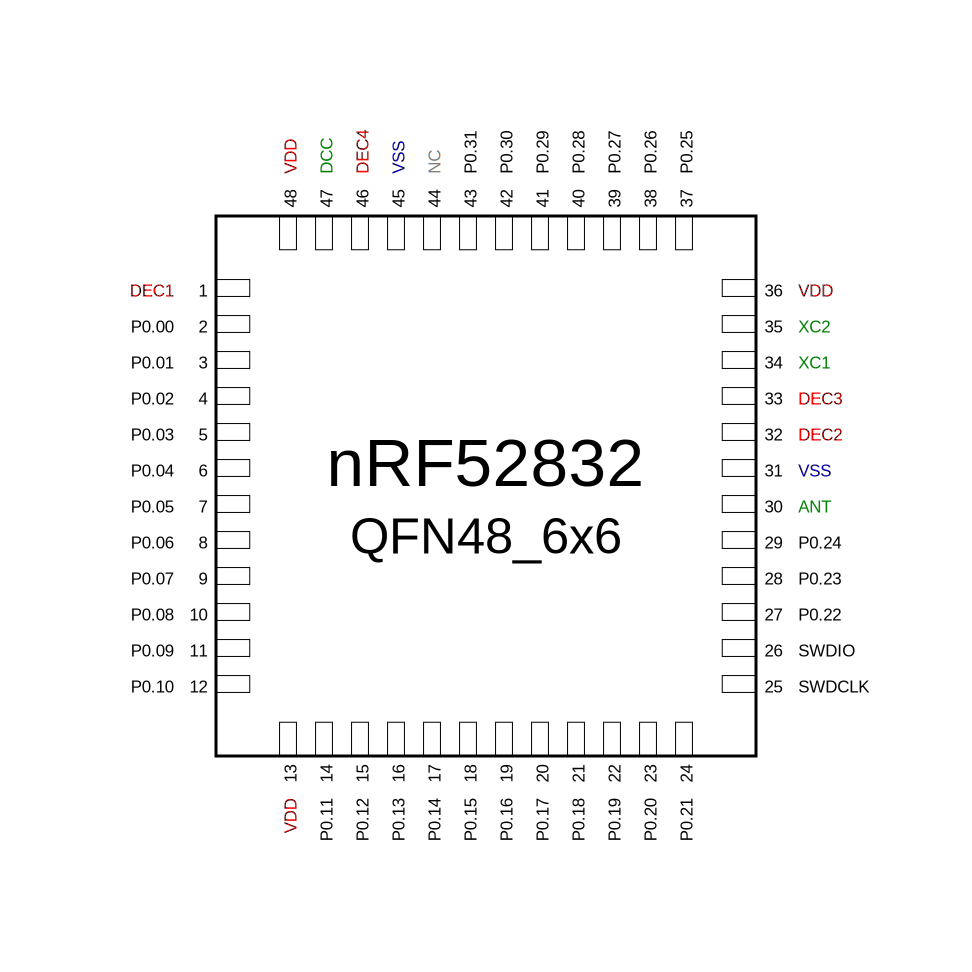
\includegraphics[width=3.3in]{qfn48}}
  \caption{Quad Flat No-Lead package outline of Nordic's nRF52832. Blue is
    ground, red is power, green is analog and black is digital input/output.}
\label{fig_qfn}
\end{figure}


% -----------------------------------------------------------------
\section{Purpose}
% -----------------------------------------------------------------
All integrated circuits are made for a purpose. An integrated circuit is like an advanced tool.
Maybe your customer want to control a sensor, charge a battery, turn on a light, or connect to the internet. An
IC help them do that. Remember this. If you don't know the purpose of the circuit that you're making,
then you need to figure out what the purpose is. There is always a purpose.


% -----------------------------------------------------------------
\section{Skills}
% -----------------------------------------------------------------
The integrated circuit in figure \ref{fig_qfn} is split into multiple levels of
hierarchy.

\begin{itemize}
  \item Infrastructure - Power management, reset, bias, clocks
  \item Domains - CPUs, peripherals, memories, bus systems
  \item Sub-systems - Radio's, analog-to-digital converters, comparators
  \item Blocks - Analog Radio, Digital radio baseband
  \item Modules - Transmitter, receiver, de-modulator, timing recovery
  \item Designs - Opamps, current-mirrors, adders, inverters, random access
        memory blocks, standard cells
  \item Devices - metal-oxide transistors, bipolar transistors, capacitors,
        resistors, diodes, inductors, thyristors
  \item Technology - n-diffusion resistors, p-diffusion resistors,
        poly-resistors, unscilicided poly resistors, metal resistors
\end{itemize}

The hierarchy levels need different skills, usually split into
analog, digital, signal processing, and firmware. Some functions, like a Bluetooth Low Energy Radio
, need all four to work. Others, like
infrastructure (power management, clocks), might not need signal processing or
software to operate.
There are extremely few analog blocks that don't have any digital input, or
digital output.

%Probably one of the only ones without digital input is the reset
%block, which serve one purpose, and one purpose only. The reset ensures that if
%the power supply is too low, the digital circuit does not start. As we will see,
%all logic gates need a minimum supply voltage to operate. But when you connect
%the battery, the voltage on the IC is 0 V, and it takes some time before the voltage
%reaches 3.0 V, so in the beginning the digital do not work. That's where reset
%circuit come in. They are made to ``work'' from 0 V.

It is rare to find one person doing firmware, signal processing, digital design, and analog design.
I know of a handful among the 1000 employees in Nordic Semiconductor that have
that ability. Usually, people are drawn to one of the four skills. Some of you
may choose not to learn any of the skills, and that's OK, but you probably won't
end up working on design of integrated circuits.

I don't know what it is, and I have no evidence to back this up, but if I
brutally generalize it seems to me that:
\begin{itemize}
\item Digital - People that like details, a sense of control, knowing that what
        they make can be verified, people that like a true/false world.
\item Signal Processing - People in love with mathematics, they can prove that the design they are making is optimal.
\item Analog - People that are fine with gray zones, not knowing, not
        understanding. People that love physics, are tolerant towards change and
        challenges to world view. They know that all models for simulation are
        wrong, but some are useful.
\item Firmware - People that like systems, and working close to end product.
\end{itemize}

% -----------------------------------------------------------------
\section{What}
% -----------------------------------------------------------------
In this course we'll focus on two areas, analog and digital.

% -----------------------------------------------------------------
\subsection{Analog}
% -----------------------------------------------------------------
Full disclosure. I'm an analog designer, I've designed analog-to-digital converters
on ICs that have now sold in the billions of devices. Since I'm an analog designer, much of what I say will be
colored by that.

The real world is analog. The real world has voltages, currents, fields,
charges, all quantities that are for most purposes continuous in time and value.
A few integrated circuits are pure analog, like the LM741 operational
amplifier. Most integrated circuits are mostly digital. But all commercial digital
integrated circuits have analog circuits inside them. Someone must make the
voltages, clocks, and everything the digital needs to talk to the outside world.
In this course we'll cover
\begin{itemize}
  \item Devices - diodes, bipolars, transistors, capacitors, resistors,
        inductors
  \item How ICs are manufactured
  \item Basic transistor configurations, and their purpose.
\end{itemize}

% -----------------------------------------------------------------
\subsection{Digital}
% -----------------------------------------------------------------
Full disclosure. I've never done digital design in Verilog on a volume product, only on
test-chips. But I know what you'll learn  in this course, which is how
to combine transistors into gates, data-paths and state machines. As for the verilog coding, all we'll do
this semester is introduce the concept to you, so what I know is plenty.
In this course we'll cover
\begin{itemize}
  \item Digital Gates
  \item Sequencing
  \item Data-paths
  \item Memories
  \item Packaging, Power, Clock, I/O
  \item Methodology
  \item Verilog
\end{itemize}

% -----------------------------------------------------------------
\section{Conclusion}
% -----------------------------------------------------------------
I hope that after this course you will know better the fundamental skill
required for integrated circuit design. This is only the start of the journey
though, and if it's hard to see where the journey will end, then remember to ask
questions, and I'll put it into context.

\begin{thebibliography}{1}
  \providecommand{\url}[1]{#1}

  \bibitem{bbs47}
  Brittain, Bardeen, Shockley ``Point-contact transistor'', online:\url{https://en.wikipedia.org/wiki/Transistor}




\end{thebibliography}






\end{document}
